% separacion_canales_bayer_tikz.tex
% Gráfica TikZ de la separación de canales en patrón Bayer - Versión exacta

\begin{figure}[h]
\centering
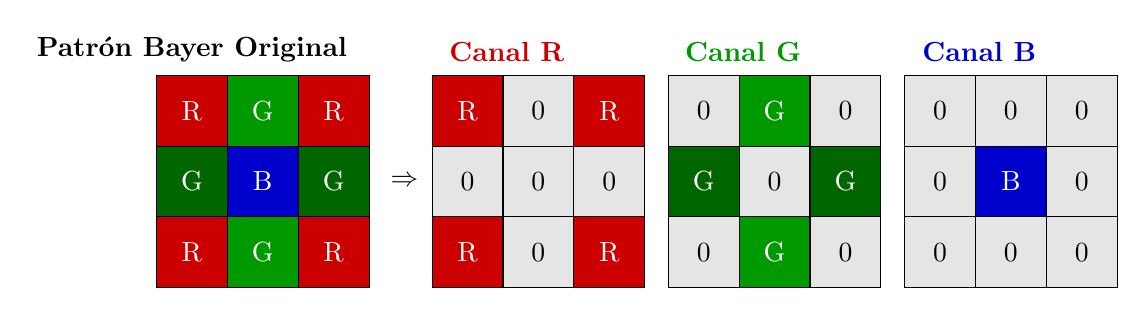
\begin{tikzpicture}[
    font=\normalsize,
    cell/.style={rectangle, draw=black, minimum size=0.9cm, inner sep=0}
]

% ============================================
% PATRÓN BAYER ORIGINAL 3×3
% ============================================

% Título
\node[above, font=\bfseries] at (0, 2.5) {Patrón Bayer Original};

% Fila 1: R G R
\node[cell, fill=red!80!black] at (0, 2) {\textcolor{white}{R}};
\node[cell, fill=green!60!black] at (0.9, 2) {\textcolor{white}{G}};
\node[cell, fill=red!80!black] at (1.8, 2) {\textcolor{white}{R}};

% Fila 2: G B G
\node[cell, fill=green!40!black] at (0, 1.1) {\textcolor{white}{G}};
\node[cell, fill=blue!80!black] at (0.9, 1.1) {\textcolor{white}{B}};
\node[cell, fill=green!40!black] at (1.8, 1.1) {\textcolor{white}{G}};

% Fila 3: R G R
\node[cell, fill=red!80!black] at (0, 0.2) {\textcolor{white}{R}};
\node[cell, fill=green!60!black] at (0.9, 0.2) {\textcolor{white}{G}};
\node[cell, fill=red!80!black] at (1.8, 0.2) {\textcolor{white}{R}};

% ============================================
% FLECHA DE SEPARACIÓN
% ============================================
\node at (2.7, 1.1) {$\Rightarrow$};

% ============================================
% CANAL ROJO (R)
% ============================================

% Título
\node[above, font=\bfseries, red!80!black] at (4, 2.5) {Canal R};

% Fila 1: R 0 R
\node[cell, fill=red!80!black] at (3.5, 2) {\textcolor{white}{R}};
\node[cell, fill=gray!20] at (4.4, 2) {0};
\node[cell, fill=red!80!black] at (5.3, 2) {\textcolor{white}{R}};

% Fila 2: 0 0 0
\node[cell, fill=gray!20] at (3.5, 1.1) {0};
\node[cell, fill=gray!20] at (4.4, 1.1) {0};
\node[cell, fill=gray!20] at (5.3, 1.1) {0};

% Fila 3: R 0 R
\node[cell, fill=red!80!black] at (3.5, 0.2) {\textcolor{white}{R}};
\node[cell, fill=gray!20] at (4.4, 0.2) {0};
\node[cell, fill=red!80!black] at (5.3, 0.2) {\textcolor{white}{R}};

% ============================================
% CANAL VERDE (G)
% ============================================

% Título
\node[above, font=\bfseries, green!60!black] at (7, 2.5) {Canal G};

% Fila 1: 0 G 0
\node[cell, fill=gray!20] at (6.5, 2) {0};
\node[cell, fill=green!60!black] at (7.4, 2) {\textcolor{white}{G}};
\node[cell, fill=gray!20] at (8.3, 2) {0};

% Fila 2: G 0 G
\node[cell, fill=green!40!black] at (6.5, 1.1) {\textcolor{white}{G}};
\node[cell, fill=gray!20] at (7.4, 1.1) {0};
\node[cell, fill=green!40!black] at (8.3, 1.1) {\textcolor{white}{G}};

% Fila 3: 0 G 0
\node[cell, fill=gray!20] at (6.5, 0.2) {0};
\node[cell, fill=green!60!black] at (7.4, 0.2) {\textcolor{white}{G}};
\node[cell, fill=gray!20] at (8.3, 0.2) {0};

% ============================================
% CANAL AZUL (B)
% ============================================

% Título
\node[above, font=\bfseries, blue!80!black] at (10, 2.5) {Canal B};

% Fila 1: 0 0 0
\node[cell, fill=gray!20] at (9.5, 2) {0};
\node[cell, fill=gray!20] at (10.4, 2) {0};
\node[cell, fill=gray!20] at (11.3, 2) {0};

% Fila 2: 0 B 0
\node[cell, fill=gray!20] at (9.5, 1.1) {0};
\node[cell, fill=blue!80!black] at (10.4, 1.1) {\textcolor{white}{B}};
\node[cell, fill=gray!20] at (11.3, 1.1) {0};

% Fila 3: 0 0 0
\node[cell, fill=gray!20] at (9.5, 0.2) {0};
\node[cell, fill=gray!20] at (10.4, 0.2) {0};
\node[cell, fill=gray!20] at (11.3, 0.2) {0};

\end{tikzpicture}
\caption{Separación de canales en patrón Bayer 3×3. El patrón original se descompone en tres matrices que muestran la información de cada canal por separado. Los ceros (gris) indican ausencia de información en esa posición para el canal correspondiente.}
\label{fig:separacion_canales_bayer}
\end{figure}
